\documentclass[a4paper,landscape,10pt]{article}

\usepackage[margin=1cm]{geometry}
\usepackage{multicol}
\usepackage{graphicx}
\usepackage{titlesec}
\usepackage{enumitem}
\usepackage{xcolor}

% Section formatting
\titleformat{\section}
{\large\bfseries\color{blue}}{}{0em}{}

\setlength{\parindent}{0pt}
\setlength{\parskip}{0pt}

\begin{document}

% -------- HEADER WITH LOGO --------
\noindent
\begin{minipage}{0.1\textwidth}
    % Please place a 'logo.png' in the documentation folder for the institution logo, or remove this line.
    \includegraphics[width=0.8\linewidth]{logo.png} 
\end{minipage}
\hfill
\begin{minipage}{0.9\textwidth}
    \centering
    {\LARGE \bfseries Causal Multimodal Medical Modelling System} \\[0.1cm]
    {\large Department of Computer Science and Engineering, FISAT}
\end{minipage}
\vspace{0.1cm}
\hrule
\vspace{0.2cm}

% -------- CONTENT IN 3 COLUMNS --------
\begin{multicols}{3}
\small % Reduce font size to fit A4 neatly

% -------- INTRODUCTION --------
\noindent\begin{minipage}{\linewidth}
\section*{Introduction}
\begin{itemize}[leftmargin=*, noitemsep, topsep=0pt]
\item \textbf{Background}: ICUs generate vast multimodal data (vitals, labs, imaging, notes). 
\item \textbf{Importance}: Holistic synthesis is vital for early patient deterioration detection.
\item \textbf{Challenges}: Existing models struggle to fuse temporal and spatial data inherently missing in clinical records.
\item \textbf{Objective}: Engineer a causally-aware deep learning framework to aggregate multimodal data for severity clinical inferencing.
\end{itemize}
\end{minipage}

\vspace{0.3cm}

% -------- ARCHITECTURE --------
\noindent\begin{minipage}{\linewidth}
\section*{System Architecture}
\begin{center}
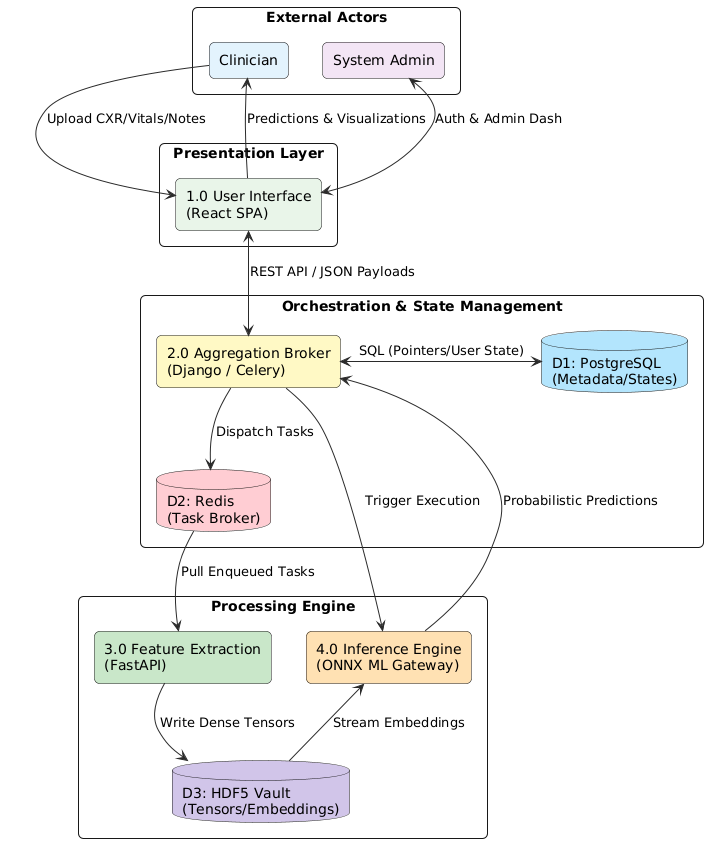
\includegraphics[width=0.7\linewidth]{UML_Diagrams/DFD_Level1.png}
\end{center}
\begin{itemize}[leftmargin=*, noitemsep, topsep=0pt]
\item \textbf{Decoupled Extraction}: FastAPIs independently process physiological measurements, text, and images.
\item \textbf{Message Brokering}: Redis orchestrates asynchronous Celery tasks without UI blocking.
\end{itemize}
\end{minipage}

\vspace{0.3cm}

% -------- PROPOSED SYSTEM --------
\noindent\begin{minipage}{\linewidth}
\section*{Proposed System}
\begin{itemize}[leftmargin=*, noitemsep, topsep=0pt]
\item \textbf{Overview}: Django-React framework integrating Transformer and CNN subgraphs.
\item \textbf{Key Features}: Time-window batching and causal-masked attention modeling.
\item \textbf{Advantages}: Resilient scaling and graceful operation against missing data.
\item \textbf{Stack}: Python, React.js, PostgreSQL, Redis, Celery, ONNX Runtime.
\end{itemize}
\end{minipage}

\vspace{0.3cm}

% -------- USE CASE --------
\noindent\begin{minipage}{\linewidth}
\section*{Use Case Diagram}
\begin{center}
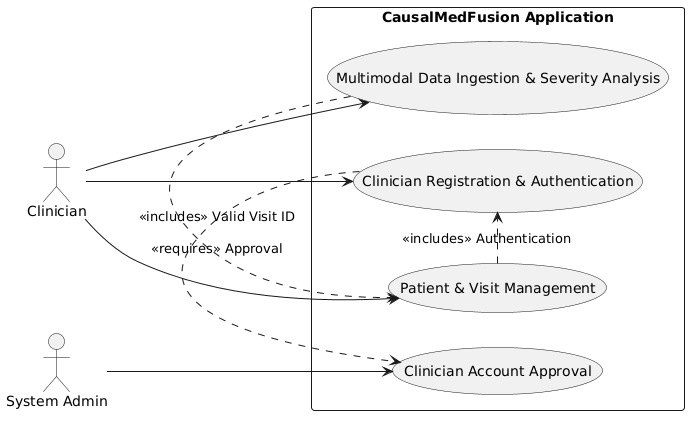
\includegraphics[width=0.85\linewidth]{UML_Diagrams/UseCase.png}
\end{center}
\begin{itemize}[leftmargin=*, noitemsep, topsep=0pt]
\item \textbf{Actors Involved}: Clinicians, System Administrators.
\item \textbf{Core Interactions}: Authenticating, managing records, uploading artifacts, viewing severity trajectories.
\end{itemize}
\end{minipage}

\vspace{0.3cm}

% -------- RESULTS --------
\noindent\begin{minipage}{\linewidth}
\section*{Results}
\begin{center}
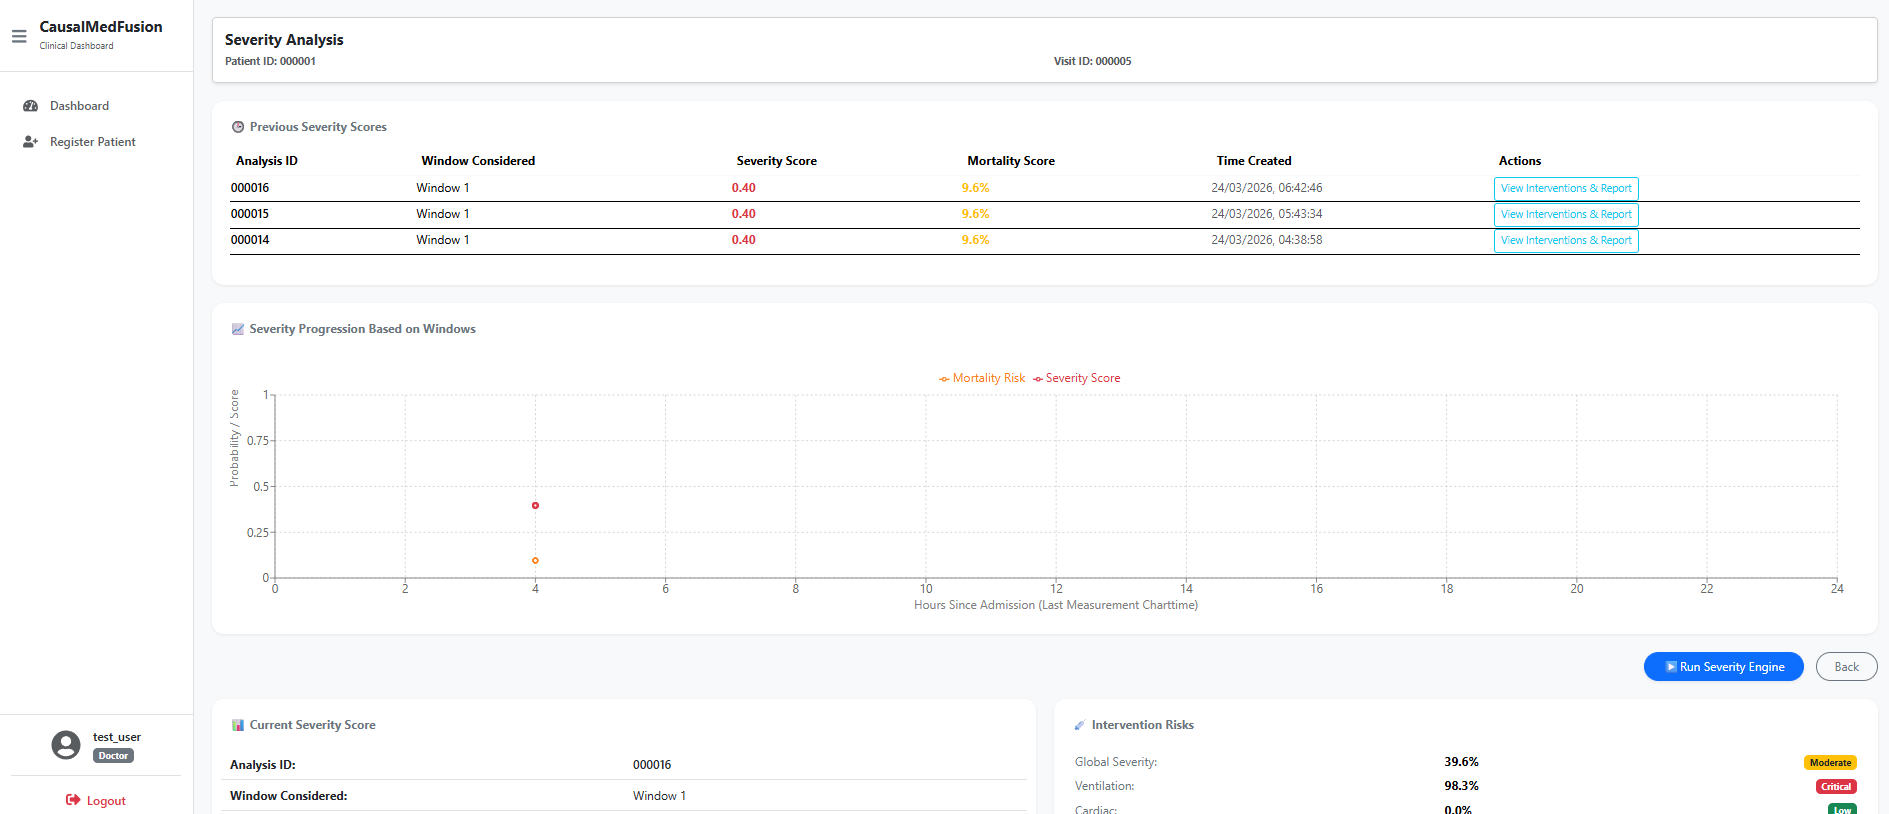
\includegraphics[width=0.85\linewidth]{screenshots/SeverityAnalysisPage.png}
\end{center}
\begin{itemize}[leftmargin=*, noitemsep, topsep=0pt]
\item \textbf{Interactive Trajectories}: Dynamic rendering of unified severity scores across time-windows.
\item \textbf{Intervention Risks}: Normalized probabilities predicting Mortality and Ventilation needs.
\item \textbf{System Resilience}: High-throughput asynchronous batching operates without failing under stress.
\end{itemize}
\end{minipage}

\vspace{0.3cm}

% -------- CONCLUSION --------
\noindent\begin{minipage}{\linewidth}
\section*{Conclusion}
\begin{itemize}[leftmargin=*, noitemsep, topsep=0pt]
\item Successfully unified unstructured notes with formatted physiological arrays.
\item Scalable microservices incorporate an ONNX Gateway resilient to data sparsity.
\item Delivered an interactive UI providing actionable prognostics for rapid patient triage.
\end{itemize}
\end{minipage}

\vspace{0.3cm}

% -------- FUTURE SCOPE --------
\noindent\begin{minipage}{\linewidth}
\section*{Future Scope}
\begin{itemize}[leftmargin=*, noitemsep, topsep=0pt]
\item \textbf{Expanded Signals}: Support continuous waveform inputs (ECG/telemetry streams).
\item \textbf{Explainable AI}: Implement explicit SHAP attention-visualization over Chest X-Rays.
\item \textbf{Federated Integration}: Broaden deployment to multi-region hospital databases.
\end{itemize}
\end{minipage}

% -------- FOOTER (TUCKED INTO LAST OPEN SLOT) --------
\vspace{0.5cm}
\begin{flushright}
\textbf{Team Members:} \\
Anuroop P V (FIT23CSD015) \\[0.3cm]

\textbf{Guide:} \\
Ms. Sheelu Susan Mathews
\end{flushright}

\end{multicols}

\end{document}